\documentclass[draftmode,draftwater]{memarticle}
% \documentclass{memarticle}
\usepackage{paralist}
\usepackage[T1]{fontenc}
\usepackage{palatino%
           , pxfonts%
           , mathpazo%
	   }
\maxtocdepth{chapter}

% ------------------------------------------------------------

% Document title control. Change these as appropriate for your document.
% ------------------------------------------------------------
\newcommand{\doctitle}{CosmoSIS \\ Introduction and Goals}
\newcommand{\brieftitle}{CosmoSIS Introduction}
\newcommand{\authors}{\href{mailto:jbk@fnal.gov,paterno@fnal.gov}%
  {Jim Kowalkowski and Marc Paterno \\ \textit{Computing Division} \\
    \textit{SSI Group}}}

\newcommand{\docversion}{3}

% ------------------------------------------------------------
%  Define new commands here
% ------------------------------------------------------------
\newcommand{\prog}[1]% format to be used for program names
  {\texttt{#1}}
\newcommand{\facs}{\name{FACS}\xspace}
\newcommand{\cosmosis}{\name{CosmoSIS}\xspace}
\newcommand{\despipe}{\name{des-pipe}\xspace}

% ------------------------------------------------------------
%  Document starts here
% ------------------------------------------------------------
\listfiles
\begin{document}
	
\topmatter % include this to typeset the title, authors, and toc.

% ------------------------------------------------------------
\chapter{Introduction\label{ch:introduction}}

\section{Rationale\label{sec:rationale}}

The dark energy science analysis done by DES will involve a large enough
group of physicists that independent and uncoordinated development will
be inefficient. In order to avoid duplicated effort, and to allow DES
members to collaborate more easily, we propose the development of an
organized environment for cosmological parameter estimation.

At the highest level, the goal of this effort is to create a
collaborative environment in which dark energy science
analysis\footnote{This effort will begin by focusing on Markov Chain
  Monte Carlo likelihood sampling analyses.} can be performed, while
helping to assure that appropriate recognition is given to the
scientific contributions of those sharing their software through this effort.
The
environment should be easy to deploy to a new computer, as long as the
computer is running one of the experiment-supported operating systems.
It should be easy for a physicist to introduce new physics algorithms or experimental datasets
into the parameter estimation process, or to replace an existing
algorithm by a different implementation. It should be easy to migrate
existing code to build under the new system. It should also be easy to
ensure that large jobs can take advantage of parallel-processing
opportunities on multi-core machines, without requiring significant
parallel-programming experience on the part of the
physicist-programmers.

\section{Purpose\label{sec:purpose}}

This document describes the features and properties of a proposed
software system, containing several elements:
\begin{inparaenum}[(a)]
\item a framework for the construction of runtime-configurable,
  parallel-capable, sampling-based parameter estimation programs, which
  we call \cosmosis (Cosmological Survey Inference System). This
  framework is initially targeted for the Dark Energy Survey
  (DES)\cite{des} project,
\item software libraries to support assembly of applications using this
  framework, and
\item a development environment to assist with collaborative development
  of such libraries, including repository use, software packaging, and
  deployment of packaged software.
\end{inparaenum}

\cosmosis will support parallel execution through a multi-process (as
opposed to multi-threaded) model, while still allowing (but not
requiring) individual bodies of code to be internally multi-threaded.
This will allow users of the framework to take advantage of modern
multi-core platforms, without requiring that physicists---who program
the modules that run within the framework---deal with the intricacies of
multi-threaded programming.

The major purpose of this document is to provide a clear description of
the project and to obtain agreement on its constraints, essential
requirements, and current state. The later sections will propose a
high-level design of the system that will meet the overall goals.

% It is the result of two days' discussion between the authors, Scott
% Dodelson (Fermilab), Elizabeth Buckley-Geer (Fermilab), and Joe Zuntz
% (Oxford), which took place August~1--2, 2012.

This document is intended for all the stakeholders in the project, as
well as for potential users of the software described.

% Describe what it is this report is going to convey or what this paper
% is about. Define the system that is being described and interesting
% qualities such as whether or not it is a utility to be shared by many.
% Include what this report should not include.

\section{Scope\label{sec:scope}}

This document describes the primary aspects of the proposed software
products and practices for using them. These include:

\begin{itemize}

\item A modular software \emph{framework} (\cosmosis) for building
  \emph{MCMC-based parameter estimation programs} for dark energy
  science. This framework will be suitable for use by physicists
  participating in the Dark Energy Survey, and eventually by others as
  well. The framework will be developed under the DOE Computational HEP
  \facs proposal. It will support the development, configuration and use
  of user-supplied MCMC samplers, likelihood calculators, and physics
  calculators.

\item A collection of application programming interfaces (APIs) that
  define how the modular elements of the framework program are
  configured, how they obtain their input data, how they interact, and
  how new modular components can be added to the system.

  Module types include \emph{samplers}, \emph{physics calculators}, and
  \emph{likelihood calculators}. The module API will support
  multi-threaded operation.

  % Per email from Joe Zuntz, support of legacy stand-alone calculators
  % is not needed.
  % Standard physics calculator modules will be
  % provided to support legacy stand-alone programs, using multi-process
  % parallelism. \ifixme{Is there also a need for a standard likelihood
  % module, to invoke legacy stand-alone likelihood calculation
  % programs?}

  APIs for physics modules, likelihood modules, and samplers will be
  provided in \cpp{}11, C99\footnote{C99 is chosen, rather than C11, for
    better compatibility with \cpp{}11; the C99 standard is part of the
    \cpp{}11 standard.}, Fortran 90, and Python 2.7.

\item A system for organizing and maintaining source control over the
  software produced by DES for this purpose. The \cosmosis framework
  code itself will reside in one repository. For each package of related
  modules, a separate source code repository will be created.

\item A system for building and testing of the source code over which we
  have control.\footnote{Third-party libraries will be built using their
    own build systems, and delivered through our product delivery
    system.} Because Python has a native build system, and a widely
  popular testing system, the system used for building and testing
  Python may be different from the system used for building and testing
  code in the compiled languages.

\item A system for recording the names, institutional affiliations, and
  other pertinent information of contributing scientists, and of
  assuring that suitable citation notices, \etc., are displayed when
  contributed code is used. The relevant information should also be
  stored in the data files produced by the system.

\item A system for distribution of software used by \cosmosis, including
  software written by DES and software written by others and used by
  \cosmosis (\eg, the GNU compiler suite, the Python interpreter, and
  \name{NumPy}~\cite{numpy}).

\item A system for organizing the data files used as input for the
  parameter estimation process.

\item A system for structuring the output files of the parameter
  estimation process. This structured output includes a scheme for
  automatic tracking of the provenance of the generated samples.

\end{itemize}

% Indicate the boundaries of this subsystem and also for this report.
% This section includes information about what is covered in the report
% and examples of what is not.

\section{Terminology\label{sec:terminology}}

In this section, we introduce some technical terminology used elsewhere
in the document.

\begin{description}

\item[Application programming interface] An \emph{application
    programming interface} (API) is a set of data structure and function
  signature definitions, along with the specification of the behavior of
  the functions.

\item[Configuration file] A \emph{configuration file} is file (usually a
  text file) that provides parameters necessary for the execution of a
  program. These are sometimes called \emph{initialization files}.

\item[Development environment] The \emph{development environment}
  comprises a set of tools (compilers, interpreters, source code
  management tools, \etc.,) used for software development, as well as a
  set of environment variables and possibly scripts used during the
  development of software. The purpose of providing a development
  environment is to help make it easy to assure that software written by
  one developer is easy for another developer to build. Compare with
  \emph{runtime environment}.

\item[Distribution system] A (binary) \emph{distribution system} is a
  means for the delivery of \emph{libraries}, \emph{programs},
  \emph{modules} and \emph{headers} (and possibly other associated
  artifacts, such as configuration files), to users. Contrast with a
  \emph{repository}.

\item[Dynamic library] A \emph{dynamic library} is a \emph{library} that
  is linked with at run-time, as opposed to (static) linking time. The
  use of dynamic libraries allows some functions of a program to be
  replaced without rebuilding the entire program.

\item[External product] An \emph{external product} is a body of software
  used by another software product, but which is not built as part of
  that other product.

\item[Framework] A \emph{framework} is a software system used to create
  a program for a specific purpose. A framework typically provides a
  means to allow the integration of user-written code into the program,
  often as \emph{dynamic libraries}. A framework typically provides the
  \code{main} function for the program. Contrast with a \emph{toolkit}.

\item[Header] A \emph{header} is a source code file, used in C and \cpp,
  to introduce prototypes of functions and definition of \code{struct}s
  or \code{class}es. In \cpp, some codes (\eg, template-based
  ``libraries'') consist entirely of headers.

\item[Installed products repository] A location (typically a directory
  tree) in which are put already-built \emph{products}, and which are
  therefore available for ``setup'' and use. Compare with \emph{source
    code repository} and \emph{product distribution repository}.

\item[Library] A \emph{library} is a body of compiled code, encompassing
  a collection of functions intended for use in building other libraries
  or programs.

\item[Likelihood calculator] A \emph{likelihood calculator} is a module
  that has the purpose of calculating, based on the values if its
  \emph{input} physics quantities, a probability associated with those
  quantities. See also \emph{physics calculator}.

\item[Module] A \emph{module} is a body of code which presents a set of
  classes, or functions, or both. Modules can consist of pure Python (in
  which case no platform dependence in the build will appear), or as
  compiled extension modules (in which case the built module is
  platform-dependent), or as a mixture of the two.

\item[Physics calculator] A \emph{physics calculator} is a module that
  has the purpose of calculating, based on the values if its
  \emph{input} physics quantities a set of \emph{derived} physics
  quantities (\eg spectra). See also \emph{likelihood calculator}.

\item[Pipeline] A \emph{pipeline} is the result of
  configuring the framework with the set of likelihood and physics
  calculators necessary to perform a specific task; it is a fully
  configured framework program.

\item[Platform] A \emph{platform} is a particular combination of
  computing hardware and operating system version. It includes many
  ``standard'' tools, \eg, \code{make}.

\item[Product] A \emph{product} is a cohesive body of software that is
  delivered to its users as a unit. It might contain one or more
  libraries or modules (to be used to build other software), or one or
  more programs, made available to the users of the product, or both. A
  product may also contain documentation, data, and other files.

\item[Product distribution repository] A location (often a web server)
  from which distribution tarballs for pre-built products are available.
  Products can not be used directly from a product distribution
  repository; they must be downloaded and then installed into an
  installed products repository.

\item[Production release] A \emph{production release} is a release of a
  body of software that has been validated through whatever mechanism is
  established for doing so. Each production release of a given body of
  software is given an identifying \emph{tag} or \emph{version number}.

\item[Program] A \emph{program} is a utility to be invoked from the
  command line, or as part of a batch job. It may be compiled (as are
  Fortran and C programs) or interpreted (as are Python programs).
  Contrast with a \emph{library}.

\item[Runtime environment] The \emph{runtime environment} comprises a
  set of tools (\eg., the commands used to obtain access to the correct
  version of installed products) used for running \prog{cosmosis} and
  related programs. It includes a set of environment variables and
  possibly scripts used to run the software. The purpose of providing a
  runtime environment that is distinct from the development environment
  is to allow software to run in environments where the build tools are
  not available, for example in environments where cross-compilation is
  needed, as is sometimes the case at supercomputing facilities. Compare
  with \emph{development environment}.

\item[Source code repository] A \emph{source code repository} is a
  system used for the version control of source code. Contrast with a
  \emph{installed products repository} and \emph{production distribution
    repository}. When the word repository is used alone, this is the
  most common meaning.

\item[Toolkit] A \emph{toolkit} is a software system, typically a
  library, module, or set of libraries or modules or both, that provides
  utilities (functions, \code{struct}s, and \code{class}es) to be used
  by user-written code. Contrast with a \emph{framework}.

\end{description}

\chapter{Essential features}

Here we describe the various aspects of the software system, the
essential functions that it must support, and the constraints to which
is must adhere. In earlier proposals and discussions, we have referred
to this this project as a framework. It is, however, more appropriately
called a system since it also encompasses developing and running the
applications that use the libraries and software modules. This section
contains rules and mandates that we must follow (constraints) and
essential functions that the system must carry out (functional
requirements).

\section{Roles that people play}

Here we focus on who makes use of this system and what sort of
activities they do\footnote{We do not describe the roles played by the
  developers of the underlying framework or supporting tools; those
  tasks are outside the scope of this document.}. We have identified
four main roles related to the \cosmosis software. The activities
performed by scientists acting in these roles are the primary focuses of
this project. It is important to note that the same person may, at
different times, more from one role to another. The main roles are:
\begin{description}

\item[Scientist user]: \emph{Scientist users} (henceforth just
  \emph{users}) make use of programs and libraries that are already
  installed. They configure programs, select input data sets, and run
  jobs. When doing analysis, scientists are often acting in the
  \emph{user} role. This can be true even when one is using code one has
  previously developed.


  Users need the set of programs code contained in the \emph{installed
    products repository} (see Fig.~\ref{fig:roles}); they will be made
  available through the \emph{runtime environment}, which may be
  deployed to a laptop, a small cluster, or a national facility such as
  NERSC. Installing the necessary items is the job of an \emph{install
    manager}.

\item[Scientist developer]: \emph{Scientist developers} (henceforth just
  \emph{developers} write, build, and test code, and usually make that
  code available for others to use. When acting in the developer role
  for one body of code, one is often also acting in the user role for
  other code; \eg a developer making use of a given sampler is most
  often not modifying the source code of the sampler, and would thus be
  acting in the user role in respect to the sampler.

Developers need to access the {source code repository}, which contains code developed by other scientists. Developers want to add code to this repository and also inspect other developers' source code to ensure compatibility. The {development environment} will contain all installed packages so that the developer can test test any changes made in the context of the full pipeline.

\item[Build manager]: \emph{Build managers} create ``official''
  distributions of software, and make those distributions available for
  others to obtain. They may also create site-specific builds of
  software, when necessary. %To date, the build managers have most often been the users and developers themselves.


  Build managers will manage the {product distribution repository} (adding and updating products) and they will tag releases in the source code repository.


\item[Install manager]: \emph{Installation managers} install
  ``official'' distributions of software on computing resources for
  which they are responsible. This role might be fulfilled by an
  individual supporting a group at a national laboratory or at a
  university, or by an individual installing software on a personal

  laptop or desktop.


  The Install manager will download the suite of products from the product distribution repository and install the system in the relevant environment.


\end{description}

Figure~\ref{fig:roles} illustrates the connections between these roles, and the activities
performed by people in them.
\begin{figure}
  \centering
  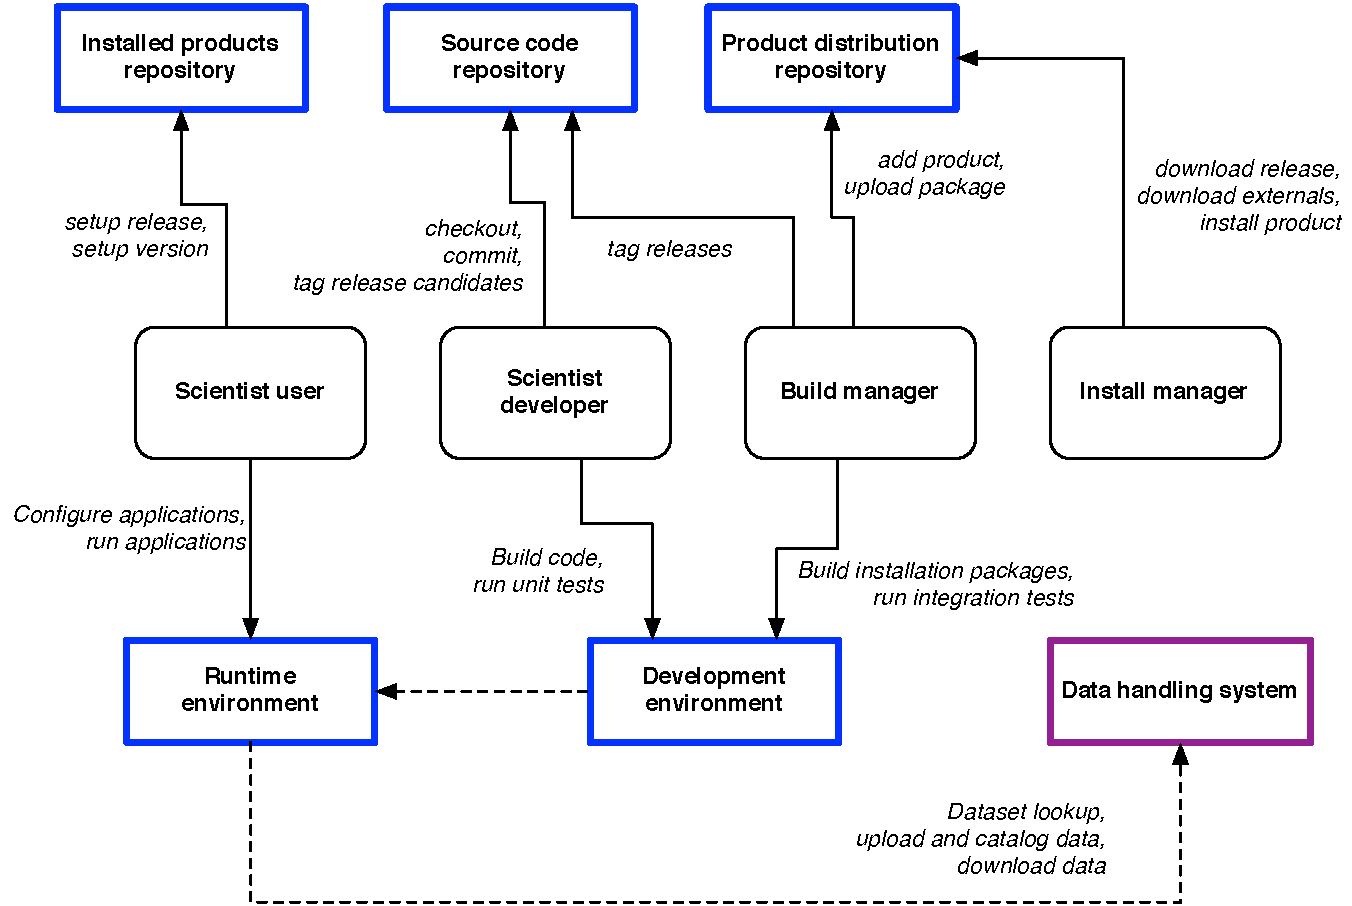
\includegraphics[width=\textwidth]{roles}.
  \caption{The roles and activities of users of the \cosmosis
    framework. Rounded rectangles denote roles; rectangles indicate
    the parts of the \cosmosis system with which a user in each role
    interacts. The labels on the arrows indicate the most important
    interactions. The dotted lines denote inclusion of one subsystem
    by another.}
  \label{fig:roles}
\end{figure}

\section{Work sequence examples}

There are several development and runtime scenarios (or work sequences)
that will help focus and describe the needs that this new system will
address.

\subsection{Configuring and running existing software}

Configuring and running existing software is done in the \emph{user}
role. Such use requires access to an installed version of the \cosmosis
software and supporting products, and also access to one or more
installed experiment-specific packages that provide the physics modules
to be used. This combination we call the \emph{runtime environment}.

A DES user would obtain access to the software by running a
DES-specific script, which ``sets up'' the runtime environment as
it will be used by DES, including a complete set of compatible products.
This makes available to the user the \prog{cosmosis} program, and also
sets up the necessary environment variables, \etc., to provide easy
access to experiment-supplied ``standard'' configuration files and
access to necessary data files.

A user would perform tasks like tailoring existing framework
configuration files to meet his specific needs, and to run the
\prog{cosmosis} program configured by such a file to produce suitable analysis
tuples.

Configuration files are text files, and can be edited by any ASCII text
editor. To run a pipeline, the user specifies the name of the
configuration file to be used. All the configuration information needed
by the program is supplied by that one file.

 For modest-size jobs, this might be done
interactively; for large-size jobs, this might involve submitting to
a batch scheduler system to execute the \prog{cosmosis} program on the user's behalf.

\subsection{Modifying an existing physics module\label{sec:modify-an-exist}}

Modifying existing physics module code is done in the
\emph{developer} role. Such use requires access to an
installed version of \prog{git}.

We propose use of the \emph{forking} workflow in use for many
git-managed software systems, as explained
in~\cite{forking-git-workflow}. This allows developers to collaborate in
their development efforts to whatever extent each is comfortable, while
allowing sufficient management of the central repository to provide the
required degree of certainty in the quality of the ``official'' releases.

The user creates a fork of the source code repository%
\footnote{Each user only needs to create a forked repository once; the
  same repository can be used for subsequent developement, including the
  creation of new physics modules, as described in
  section~\ref{sec:creating-new-physics}.}
for their modified version,
and commits changes that alter one or more of the physics modules.
Ideally some guiding documentation or script will be provided to guide
the user.

They rebuild the changed module and run some analyses on this
alternate version, perhaps comparing results from it with the
master repository.  These tests may be on a different machine if the
tests are extensive.

When they are satisfied that it works the developer issues a pull
request to the build manager to merge their changes into the master
repository.

\subsection{Creating a new physics module\label{sec:creating-new-physics}}

Creation of new physics modules in done in the \emph{developer} role.

Once again, the developers begins by creating a new fork, if needed, of the source code
repository. They then copy a template directory
that creates a stub module according to the language they want to write
in, or use a provided skeleton generator to write one.

The generated (or copied) code contains the appropriate interface
specification,
which connects the user's code to the
framework, and any additional code files necessary for the chosen language.

They then modify the module inputs and outputs in the interface file,
and add a
calculation to the primary files that does the main work of the module.
They also modify a short metadata text file to describe the
module, its authorship, inputs, outputs, and purpose.

They then proceed to test and pull-request the module as described in the
previous work sequence example.

\subsection{Creating an official release of the physics module code}

Creation of an official release is done in the \emph{build manager}
role. The times at which this is to be done should be determined by the
appropriate person or persons responsible for managing the code in
question.

The creation of an official release comprises several steps, sketched
here:
\begin{enumerate}
\item Check out the appropriate version of the source code.
\item Integrate whatever \emph{pull requests} (generated by developers
  in the steps described in
  section~\ref{sec:modify-an-exist}
  and~\ref{sec:creating-new-physics}) are to be included in the
  candidate release.
\item Tag the source code repository with the appropriate version
  number. This allows the source code used to produce the production
  release to be unambiguously identified. Note that this requires write
  access to the source code repository.
\item \label{item:build} Build the tagged version of the code on the
  platforms the build manager is supporting. Run all automated tests.
\item If the tests pass, build the distribution tarballs, and upload
  them to the product distribution repository. If the tests do no
  succeed, those responsible for the failing code should be notified so
  that they can fix their code. If necessary, the build manager may
  disable the build of specific modules in specific releases.
\end{enumerate}

Some build managers may be responsible only for building on a specific
platform, and not for tagging the code. Such a build manager would begin
at step~\ref{item:build}. Note that this task does not require write
access to the source code repository.

\subsection{Installing a new release}

Installation, on some computing hardware, of an already-built release is
done in the \emph{install manager} role. An install manager may be
responsible for a single laptop or desktop, or for a small cluster, or
for a national facility such as NERSC. The install manager for a given
machine must have appropriate permissions to manipulate the files in the
\emph{installed product repository} on that machine.

To install a new release of a given product, the install manager follows
these steps:
\begin{enumerate}
\item Download an installation tarball from the \emph{product distribution
  repository} (using a tool such as \prog{wget} or \prog{curl}).
\item Unwind the tarball into the top-level directory of the installed
  product repository.
\item If necessary, run any provided post-installation script.
\end{enumerate}

\section{Software categories}

Software added to the system falls into several categories: platform,
external, core, contributions. This section defined each of these
categories and describes their constraints and essential requirements.

These categories are arranged in a hierarchy of dependencies: platform
software can depend only on other platform software; external software
can depend upon other external software and on platform software; core
software can depend on other core software, and on external and platform
software; contribution software can depend on other contribution
software, and on anything in any of the other categories.

\subsection{Platform}

Platform software elements are those elements which are not delivered
through the software product distribution system, but are required as
part of the software inherent on a given platform. Some examples would
be the \prog{bash} shell, and the system's standard C library
(\prog{libc.so} on Linux systems, \prog{libSystem.dylib} on Darwin
systems).

\subsection{External}

External software elements are those elements distributed through the
software product distribution system, but which are not created from
software controlled by the project (\eg the Python interpreter and the
GNU Scientific Library). Typically they have their own system for
building the software.

Such software elements will be built using their own build system, and
packaged into the form used by the product distribution system.

\subsection{Core}

Core software elements are those elements that are part of the project,
and are used by scientist-developer written code, but which do not
(often) need modification by scientist developers.

\subsection{Contribution}

Contribution software elements are those elements that are part of a
collaboration's code. They are the software elements with the ``physics
knowledge'' of the system, and are primarily developed by scientists.

\section{Run-time environment}

The subsystems that permit one to use the developed software and other
externally developed applications and tools to solve problems are
contained in this section. This section defines each of these subsystems
and describes their constraints and essential requirements.

\subsection{Runtime configuration}

Runtime configuration refers to the configuration of the \prog{cosmosis}
program. Runtime configuration should be done with a text file, so that
simple text editors can be used to modify the file, and so that
configuration files can be kept in a source code repository and compared
with tools like the common Unix utility \prog{diff}.

The choice of sampler to be used in a given program execution should be
specified as part of the runtime configuration, rather than by the
choice of main program to run.

The choice of likelihood calculators and physics calculators to be run
should be determined by the configuration file. All the configuration
parameters for such modules should be specified as part of the
configuration file, and not be read from individual files by each
module. Modules should not read the configuration file themselves; they
should be given the necessary configuration parameters as early as
possible in the program, so that errors in configuration can be
diagnosed as early as possible. Errors in configuration should cause a
graceful program shutdown, accompanied by any relevant error messages.
Some configuration parameters are program-wide, while others are
module-specific. Some modules need to evaluate parameters only in order
to assure they are not outside the physical bounds within which the
module's calculations are valid. Thus is seems necessary for each module
to receive the full set of configuration parameters for the whole
program.

An important task of the runtime configuration system is the support of
provenance tracking, to help assure that the results of calculations are
reproducible. In support of this provenance tracking, modules may not
modify the configuration parameters they receive; the parameters are
read-only.

It should be possible to provide a ``standard'' configuration that
specifies sensible values for all parameters for each module. The author
of a module should supply such a configuration along with the code of
the module. It should be possible for a user to configure any module by
specifying only those parameters whose values are to be changed from the
values established by the standard configuration.

\subsection{Data repositories}

While small data sets (less than approximately 1~MB) needed by a module can
reasonably be stored in the repository in which the code is stored,
larger data files demand an alternative solution.

For the largest of data sets (greater than approximately 100~GB), it may
be unreasonable to keep many copies of the same files. For such data
sets the best solution may be to keep the files in a DES-defined
directory structure at NERSC. The use of a defined directory structure
allows some flexibility here. Parts of the directory structure can be
more replicated elsewhere, if such is needed, more cheaply than the
entire set, and code can be written to work not only at NERSC, but
anywhere that the appropriate part of the data set has been replicated.

All data repositories should be accessible using the same API, so that
the same code can be used wherever the data are available.

\subsection{Configuration repositories}

A ``standard'' configuration file for each module should be kept in the
source code repository that contains the code for that module. It should
be possible to keep other configuration files in the same repository.

Any configuration files in the source code repository should also be
shipped with a binary build of the software, so that users of the
runtime system do not require access to a copy of the source code only
for the purpose of obtaining the configuration files.

\subsection{Installed products repositories}

On centrally managed machines (\eg, university clusters or NERSC), a
repository of all available products built for that platform should be
maintained by someone with that responsibility. This task must not
require that the maintainer have elevated system privileges.

In order to facilitate individual users' ability to make use of
libraries that are not yet ``officially'' distributed, it must be
possible for a user to install his own packages without needing write
access to a centrally-managed installed product repository. The user
should be able to make his own repository, and to use products from it
in conjunction with products from the central repository.

\subsection{Environment settings}

In order to facilitate the writing of portable code (portable between
different machines, as well as between different platforms), we need a
set of cooperating scripts to establish the user's working environment.
One part of the scripts may need to be installation-specific, to
identify the locations or names of installation-specific items (such as
the location of the local installed product repository). Most of the
scripts should be installation-independent.

Ideally, users of CosmoSIS would need only to set up the CosmoSIS
product to obtain access to all necessary software. Developers using
CosmoSIS should be able to do so with a few steps as possible; setting
up the software development environment should require no more than one
command. The tools used for development must be clearly documented.

\subsection{Data handling interface}


\subsection{Platform interactions for special facilities}

At some specific facilities (\eg, NERSC), the nature of the facility
might require the use of some products that differ from those available
at other sites (\eg, the NERSC batch environment and the \emph{modules}
system used to access products).

In order to avoid users needing to learn too many sets of commands for
the same purpose, such systems should be made to operate through the
same commands as are used for the same purpose elsewhere, whenever
feasible.

The software environment established by CosmoSIS should in no way
prevent use of facility-specific features, even when it does not
directly provide any facilities for supporting such features.

\section{Development environment}

The subsystems that permit software development activities and house
software artifacts are contained in this section. This section defines
each of these subsystems and describes their constraints and essential
requirements.

\subsection{Source code repositories}

Source code that is managed by DES---specifically, the source code for
physics modules written by DES---should be kept in a source code
repository that is accessible by all members of the DES collaboration. A
git repository on BitBucket will be provided for this purpose.

Code that is not managed by DES, but is used by DES, should not reside
in this repository. Such code would include, for example, GSL, cfitsio,
and WMAP7. DES will not keep this code under revision control because
identifiable versions of the code are available from elsewhere.

The code for the \cosmosis framework itself (as opposed to the code for
the DES physics modules) will reside in a repository distinct from the
repository in which the DES physics module source code resides. This
repository is separate from the code repository in which the physics
modules resides to make it easier to release new versions of each
independently, so that development may proceed on each at its own pace.
This separation also makes it easier to see how other groups could make
use of the \cosmosis framework, even if they are doing physics analyses
distinct from those done with the DES physics modules.

\subsection{Build, test, package, and local install}

\subsection{Distribution repositories}

\section{Project-wide constraints}

\subsection{Supported platforms}

For all supported platforms, there will be regular releases of the
project's software that are centrally built and made available for
distribution. On a best-effort basis, we will try to maintain code
portability so that interested users can build their own releases on
unsupported systems, but releases for unsupported systems will not be
centrally created and distributed.

The set of supported platforms includes:
\begin{enumerate}
\item Scientific Linux Fermi 6.x, on x86-64 hardware, in 64-bit mode.
\item Scientific Linux Fermi 5.x, on x86-64 hardware, in 64-bit mode.
\item Darwin 10.x (as shipped with Mac OS~X 10.6, ``Snow Leopard''), on
  x86-64 hardware, in 64-bit mode.
\item Darwin 11.x (as shipped with Mac OS~X 10.7, ``Lion''), on x86-64
  hardware, in 64-bit mode.
\item Darwin 12.x (as shipped with OS~X 10.8\footnote{The ``Mac'' has
    apparently been dropped from the operating system name as of
    Mountain Lion.}, ``Mountain Lion''), on x86-64 hardware, in 64-bit
  mode.
\item Ubuntu 12.x~LTS ``Precise Pengolin'', on x86-64 hardware, in
  64-bit node.
\end{enumerate}

\subsection{Supported shell}

On all supported platforms, the runtime and development environments
will require use of the bash shell, version~3 or newer. This is to avoid
the need to maintain a multiplicity of scripts for these environments,
with the risk that the script might provide subtly different behavior.

\subsection{Supported compilers}

In order to assure compatibility of delivered software products, and to
allow us to upgrade our choice of compilers on our own timescale, the
build system will not make use of the platform-supplied compiler or
Python interpreter. Instead, the compiler suite and the Python
interpreter will be supplied as a UPS product, for each of the supported
platforms.

For all supported compilers, on each platform for which the compiler is
supported, there will be regular releases of the project's software that
are centrally built and made available for distribution.

The set of supported compilers includes:
\begin{enumerate}
\item The GNU \cpp{}, C and Fortran compilers, from GCC 4.7.3.
\item Python 2.7.3.
\end{enumerate}
Newer versions of the GNU compilers will be used when they become
available. Newer versions of Python 2.7 will be used when they become
available. Python 3.x will not be supported, because of its
incompatibility with some of the Python modules of interest for the
scientific community.

Non-free compilers will not be officially supported, because they can
not be freely distributed. However, on a best-effort basis, we will try
to keep the build system able to support important commercial compilers,
so that individuals or sites which have licenses to those compiler can
build the software on their own computing resources.

\subsection{Language standards}

Using defined standards for the supported languages, when possible, aids
in the portability of code, making it more certain that code written in
one environment will build and run correctly in other environments.
However, not all language standards are equivalently useful.

\subsubsection{C programming language}

For C we will support the C99 language standard. This language standard
is fully supported by the GNU compiler suite, version 4.7, and is widely
supported by other compilers as well.

\subsubsection{\cpp{} programming language}

For \cpp{} we will support the \cpp{}11 language standard, in the subset
supported by the GNU compiler suite, version 4.7. This is the newest
\cpp{} standard, and while it is not yet completely supported by any
compiler, the (large) fraction of features supported by GCC is
sufficiently valuable to be worth its use.

\subsubsection{Fortran programming language}

For Fortran, we will support Fortran~90 with the additions of TR-15581
(which adds enhanced data type facilities), plus the following list of
features from Fortran~2003:
\begin{enumerate}
\item procedure pointers,
\item IEEE exceptional values,
\item C interoperability features: the \texttt{ISO\_C\_BINDING} module
  and the \texttt{bind} and \texttt{value} attributes.
\end{enumerate}

\subsubsection{Python programming language}

For Python, we will support only the CPython interpreter (not, \eg, the
JVM-based Jython). We will support Python 2.7. On a best-effort bases,
we will try to keep code that will also be compatible with Python 3.x,
to reduce the work that would be necessary if, at some future date, the
community decides to move to using Python 3.

\section{Parallel Interfaces}

This section should document the parallel interfaces that are supported for
user-provided modules.  (OpenMP for C,C++, and Fortran, Python multiprocess? pthreads? MPI threads?).
APIs that are exposed to the user should be made thread-safe or explicitly labelled
as unsafe.

% \begin{fixme}
%   Things to discuss in this section:
%   \begin{itemize}
%   \item concepts
%   \item current system architecture
%   \item current development methods
%   \item current method of running programs
%   \item areas we discussion (tools, techniques, components)
%   \item what items are most important?
%   \item possible changes (differences between what they have and what
%     we propose)
%   \end{itemize}
% \end{fixme}

\chapter{The current situation\label{ch:current_situation}}

The current DES parameter estimation software, residing in the
\despipe repository, consists of a variety of software
artifacts, written in C99\footnote{The project makefiles typically, but
  perhaps not uniformly, set \texttt{-std=c99}.},
Fortran~90\footnote{Inspection of the source code shows use of features
  removed in Fortran~95, \eg, the \texttt{PAUSE} statement. However, the
  project makefiles do not specify a standard; thus the gfortran default
  of \texttt{-std=gnu} is used, which specifies a superset of the
  Fortran 95 standard that includes all of the extensions supported by
  GNU Fortran, although warnings will be given for obsolete extensions
  not recommended for use in new code. Elsewhere in the code is use of
  \texttt{USE ISO\_C\_BINDING}, which is a Fortran~2003 feature (and a
  GNU extension in earlier versions of gfortran). The Fortran language
  variant used in the code base is not precisely defined.}, and
Python\footnote{The project makefiles indicate a requirement of Python
  2.6 or Python 2.7.}. Some of these consist of code written by DES
members, others are code written by others in the astrophysics
community, and others are code written by those outside the community,
but all of which have been imported into the \despipe source
code repository. Some software artifacts are \emph{programs}, others are
(Python) \emph{modules}, while others are \emph{libraries}.
Figure~\ref{fig:astropackages} shows the dependencies between the
software packages currently used by DES parameter estimation programs.

\section{Current external dependencies}

Code in the \despipe repository depends upon several different
external products. These are not delivered as part of the
\despipe system; each must be installed by other means. The
required products include:
\begin{enumerate}
\item A C99 compiler.
\item A Fortran~90 compiler.
\item \name{CFITSIO}. The exact version required is unclear.
\item A Python interpreter, either version 2.6 or version 2.7. Only
  CPython can be used, because of the widespread dependence on
  \name{NumPy}, which does not support alternative Python
  implementations.
\item \name{NumPy}. The exact version required is unclear, but it must
  be built against the correct Python version. \name{NumPy} has optional
  pieces (\eg, \texttt{numpy.numarray.image}); these are not required.
\item \name{PyFITS}. The exact version required is unclear, but it must
  be build against the correct Python version.
\item \name{matplotlib}. The exact version required is unclear, but it
  must be build against the correct Python version. \name{matplotlib}
  depends upon \name{libpng} and \name{freetype}. Since this tool
  supports multiple optional user-interface toolkits, the exact set to
  be supported must be defined.
\item \name{SciPy}. The exact version required is unclear, but it must
  be built against the correct Python version and using the correct
  \cpp{} compiler. \name{SciPy} involves several other dependencies,
  which we do not elaborate further here: \name{SuiteSparse},
  \name{pcre}, and \name{swig}. \name{SciPy} has optional parts; it is
  not clear which are needed.
\item \name{FFTW?}. A common fft library (3.3 is the latest version)
\item \name{GSL?}.  The GNU scientific library.
\item \name{BLAS?}. A binary linear algebra system tuned for the local
  system and linked as appropriate to both GSL and Numpy.
\item \name{emcee}. The exact version required is unclear, but it must
  be built against the correct Python version. \name{emcee} requires
  \name{mpi4py} for full utility, but can work without it; it also
  requires \name{NumPy}. As of version 1.1, \name{emcee} is compatible
  with Python 3. The version current as May~7, 2013 is 1.2.
\item \name{PyMC}. The exact version required is unclear, but it must be
  built against the correct Python version. It requires \name{SciPy},
  \name{matplotlib}, and \name{pydot}. It seems that \name{PyMC} 2.2 and
  newer support Python 3\footnote{This is based upon commit messages in
    the PyMC project git repository.}.
\end{enumerate}

\section{Current internal dependencies}

The \despipe software is stored in a single
Mercurial\cite{mercurial} repository, hosted at
BitBucket\cite{bitbucket}. This repository includes some source code
from third parties, imported into the repository.

Figure~\ref{fig:astropackages} shows the dependency graph of the various
named products.

\begin{figure}
  \centering
    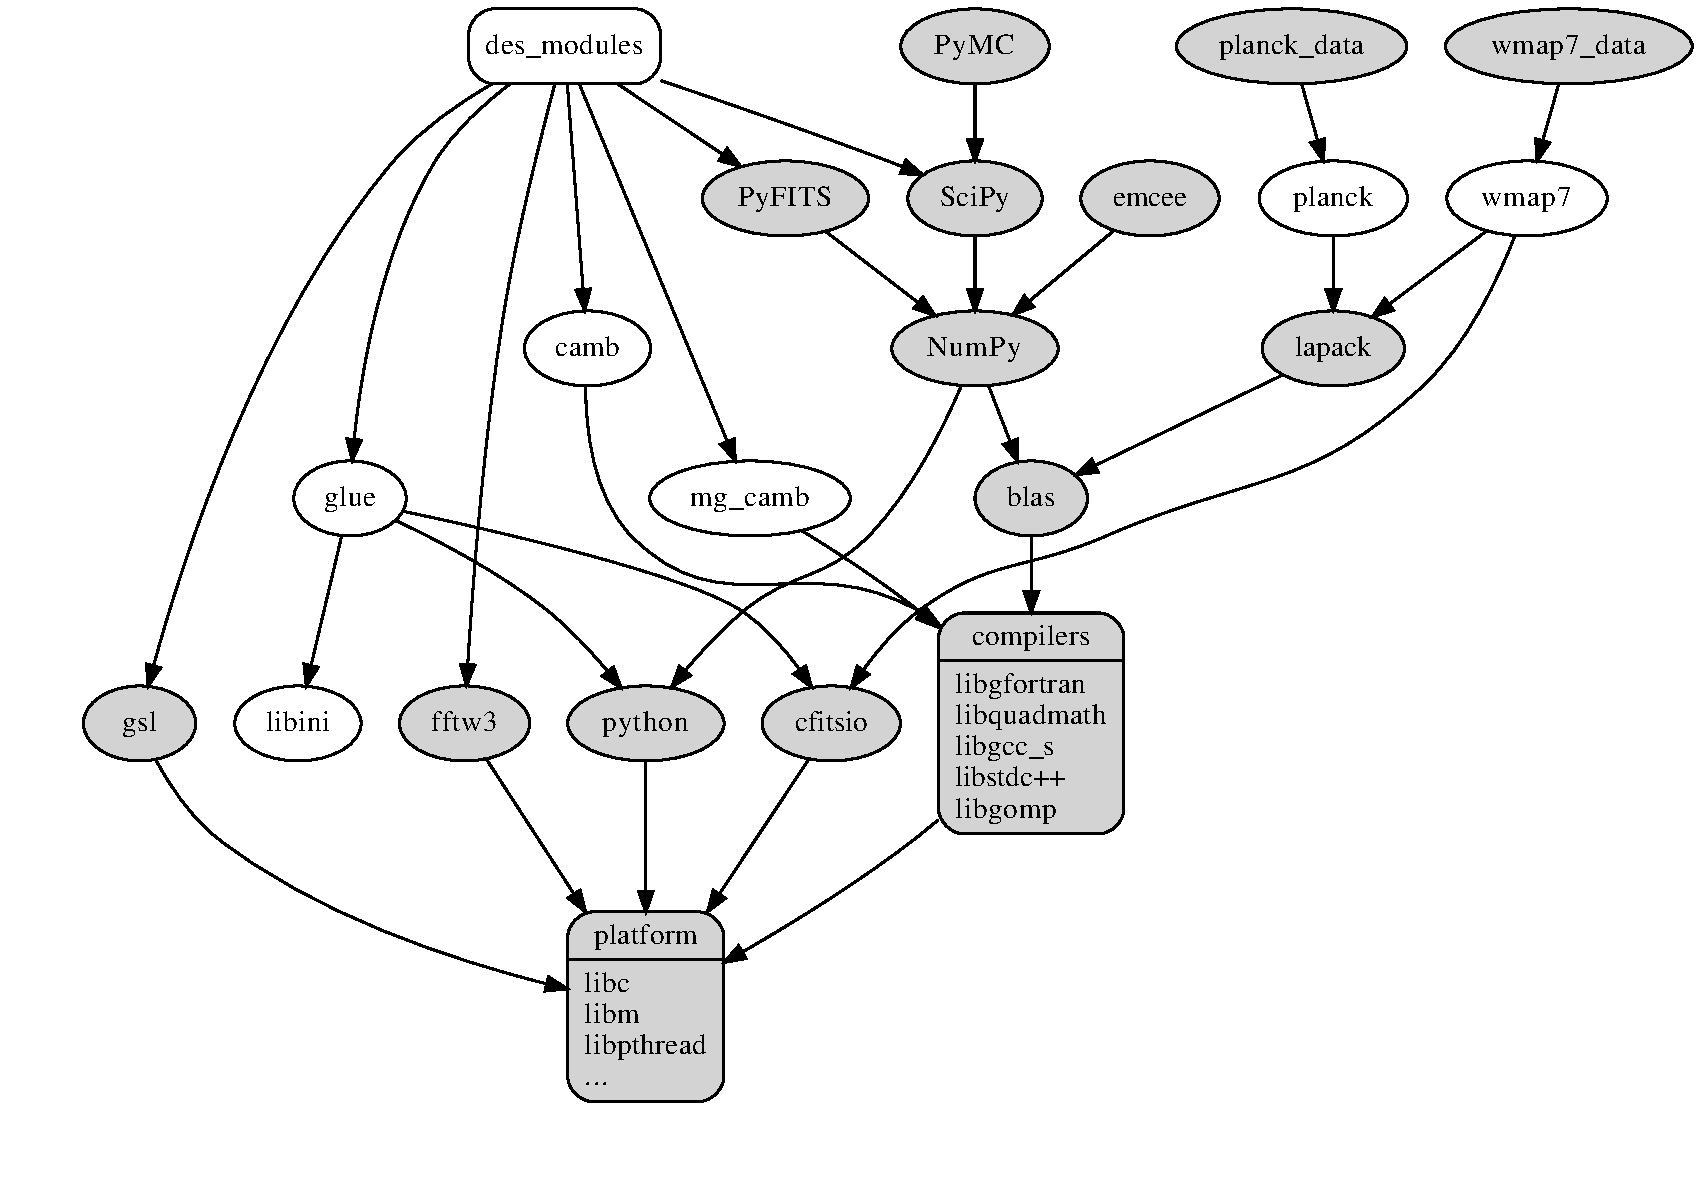
\includegraphics[height=\textheight,width=\textwidth,keepaspectratio=true]{astro_packages}
    \caption{Software packages currently part of the DES parameter
    estimation system. Rounded rectangles enclose groups of related
    code. Ellipses denote software products that are not grouped.
    Shaded shapes are used for packages that are not provided with
    \texttt{des\_pipe}; their presence must be verified by the user;
    the other software packages are present in the \texttt{des\_pipe}
    repository, and built as part of the system. \texttt{wmap7\_data}
    and \texttt{planck\_data} denote the large data files needed for
    use of their related codes. The library names listed in
    \texttt{platform} reflect Linux systems; Darwin systems have their
    equivalents.} \label{fig:astropackages}
    \begin{fixme}
    Please verify these dependencies.
    \end{fixme}
\end{figure}

\section{Current build system}

For C and Fortran code, the \despipe build system is based on
\name{make}, and consists of a set of Makefiles. For the Python code,
there is no build system; the user must have the software repository
available, and the Python environment correctly established to find the
Python modules of interest.

Building of each C or Fortran library is controlled independently, by
the individual Makefile for that module. Each Makefile can add or
replace compiler command-line switches and linker switches. This
includes control over the optimization level used by the C or Fortran
compiler, what compiler extensions are used (\eg, OpenMP), and what
preprocessor variable declarations are introduced (to control
conditional compilation of code).

There is no specific command to build all available modules. To build
each module, the user must execute the Makefile in each directory he is
interested in building. The user must have sufficient facility with
Makefile to be able to identify the targets of interest in each
Makefile.

Some Makefiles set compiler switches to values that can result in code
that is not compatible with code from other modules, \eg
\prog{shear/becker/Makefile} sets the switch \texttt{-fshort-enums},
which produces code that in not binary-compatible with code generated
without that switch.

\section{Current development techniques}

All the \despipe software (both the framework ``glue'' code and
physics module code) is maintained in a single (Mercurial) source code
repository. Additionally, some third-party code has also been copied
into the \despipe repository.

There is no official ``release procedure''; each version of the software
is identified by the Mercurial tag number in which that version of the
software can be found.

The directory structure into which the code is organized reflects both
the scientific nature of the code (\eg \prog{baryon}, \prog{boltzman})
and also the author (or at least primary author) of the code contained
in the directory.

There is little formal structure to the code; sharing of code through
use of user-written libraries is rare or non-existent. Some code sharing
is done by copying of source code, with subsequent modification. Library
use seems mostly constrained within the individual directories described
above.

There is no formal organization for running either tests of individual
algorithms (unit tests) nor for testing of full programs (integration
testing); such testing is left to the individual authors.

\section{How programs are executed in the current system}

Programs are executed by running one of the provided samplers:
\begin{enumerate}
\item \prog{sampler.py} (from \prog{sampler/pymc\_sampler}),
\item \prog{emcee\_sampler.py} (from \prog{sampler/emcee\_sampler}, or
\item \prog{emcee\_sampler\_mpi.py} (from
  \prog{sampler/emcee\_sampler}), which is launched by \prog{mpirun}.
\end{enumerate}

Runtime configuration is provided by a (text) initialization file. This
file controls all (or nearly all) of the configuration of the program.
Most importantly, it names the physics modules that are to be executed,
and names the function to be invoked for each module (although in all
cases this function name seems to be \texttt{execute}). It also provides
the configuration parameters needed by each of these physics modules, as
well as providing configuration for both the \texttt{pymc} and
\texttt{emcee} samplers. The actual sampler that is used is determined
by the program that is run, not by the configuration file.

Configuration files use some filenames that are relative to a
user-settable \emph{root} directory, and some that are relative to the
user's current working directory, which is expected to be the directory
in which the initialization file resides.

\bibliographystyle{abbrv}
\bibliography{cosmosis}


\end{document}

%%% Local Variables:
%%% mode: latex
%%% TeX-master: t
%%% End:
